\documentclass[a4paper, table]{article}
\usepackage[spanish]{babel}
\usepackage[utf8]{inputenc}
% Useful packages, sorted so packages of similar functionality are grouped together. Not all are essential to make the document work, however an effort was made to make this list as minimalistic as possible. Feel free to add your own!

% Essential for making this template work are graphicx, float, tabularx, tabu, tocbibind, titlesec, fancyhdr, xcolor and tikz. 

% Not essential, but you will have to debug the document a little bit when removing them are amsmath, amsthm, amssymb, amsfonts, caption, subcaption, appendix, enumitem, hyperref and cleveref.

% inputenc, lipsum, booktabs, geometry and microtype are not required, but nice to have.

\usepackage[utf8]{inputenc} % Allows the use of some special characters
\usepackage{amsmath, amsthm, amssymb, amsfonts} % Nicer mathematical typesetting
\usepackage{lipsum} % Creates dummy text lorem ipsum to showcase typsetting 

\usepackage{graphicx} % Allows the use of \begin{figure} and \includegraphics
\usepackage{float} % Useful for specifying the location of a figure ([H] for ex.)
\usepackage{caption} % Adds additional customization for (figure) captions
\usepackage{subcaption} % Needed to create sub-figures

\usepackage{tabularx} % Adds additional customization for tables
\usepackage{tabu} % Adds additional customization for tables
\usepackage{booktabs} % For generally nicer looking tables

\usepackage[nottoc,numbib]{tocbibind} % Automatically adds bibliography to ToC
\usepackage[margin = 2.5cm]{geometry} % Allows for custom (wider) margins
\usepackage{microtype} % Slightly loosens margin restrictions for nicer spacing  
\usepackage{titlesec} % Used to create custom section and subsection titles
\usepackage{titletoc} % Used to create a custom ToC
\usepackage{appendix} % Any chapter after \appendix is given a letter as index
\usepackage{fancyhdr} % Adds customization for headers and footers
\usepackage[shortlabels]{enumitem} % Adds additional customization for itemize. 

\usepackage{hyperref} % Allows links and makes references and the ToC clickable
\usepackage[noabbrev, capitalise]{cleveref} % Easier referencing using \cref{<label>} instead of \ref{}

\usepackage{xcolor} % Predefines additional colors and allows user defined colors

\usepackage{tikz} % Useful for drawing images, used for creating the frontpage
\usetikzlibrary{positioning} % Additional library for relative positioning 
\usetikzlibrary{calc} % Additional library for calculating within tikz

% Defines a command used by tikz to calculate some coordinates for the front-page
\makeatletter
\newcommand{\gettikzxy}[3]{%
  \tikz@scan@one@point\pgfutil@firstofone#1\relax
  \edef#2{\the\pgf@x}%
  \edef#3{\the\pgf@y}%
}
\makeatother



 % Loads in the preamble 
% Give your report a title
\newcommand\reporttitle{Trabajo de Planificación Ambiental de Proyectos}

% Insert course code, name, quartile number and year (or any other subtitle)
\newcommand\reportsubtitle{
Evaluación Ambiental de Proyectos
}

% Add your group number (for DBL) or any other text.
\newcommand\groupnumber{
\textbf{Group Number: C2566-OG0262-3476}
}

% Insert authors and student numbers here
\newcommand\reportauthors{
Isabela Arenas Escudero \\
Juan Pablo Tobón García \\
Juan Manuel Young Hoyos
}

% Add the name of your tutor (for DBL) or any other text.
\newcommand\grouptutor{
Tutor: Jose Alfredo Vasquez Paniagua
}

% Date and location (default: current date and Medellín)
\newcommand\placeanddate{
Medellín, \today
}

% Define EAFIT-blue (color of the EAFIT logo). Can be changed to drastically change the look of the template
\definecolor{EAFIT-blue}{RGB}{2, 8, 115}

% Sets up hyperlinks in the document to be colored
\hypersetup{
    colorlinks=true,
    linkcolor=EAFIT-blue,
    urlcolor=EAFIT-blue,
    citecolor = EAFIT-blue
    }
\urlstyle{same} % Defines settings for link and reference formatting

% Change bullet style for level 1, 2 and 3 respectively for itemize
\renewcommand{\labelitemi}{\scriptsize\textcolor{EAFIT-blue}{$\blacksquare$}}% level 1
\renewcommand{\labelitemii}{\scriptsize\textcolor{EAFIT-blue}{$\square$}}% level 2
\renewcommand{\labelitemiii}{\textcolor{EAFIT-blue}{$\circ$}}% level 3

% \renewcommand{\labelitemi}{\small\textcolor{EAFIT-blue}{\ding{70}}} % level 1
% \renewcommand{\labelitemii}{\small\textcolor{EAFIT-blue}{\ding{71}}}% level 2
% \renewcommand{\labelitemiii}{\tiny\textcolor{EAFIT-blue}{\ding{71}}}% level 3

% Change bullet style for level 1, 2 and 3 respectively for enumerate
\renewcommand{\labelenumi}{\textbf{\textcolor{EAFIT-blue}{\arabic*.}}}% level 1
\renewcommand{\labelenumii}{\textbf{\textcolor{EAFIT-blue}{[\alph*]}}}% level 2
\renewcommand{\labelenumiii}{\textbf{\textcolor{EAFIT-blue}{\roman*.}}}% level 3

% Have reference labels be linked to section (section 3 will have fig. 3.1 etc.)
\counterwithin{equation}{section} % For equations
\counterwithin{figure}{section} % For figures
\counterwithin{table}{section} % For tables

% Creates a beautiful header/footer
\pagestyle{fancy}
\lhead{
\includegraphics[height=14pt]{Figures/0. General/eafit_logo_blue.png}}
\rhead{\reporttitle}
\renewcommand{\footrulewidth}{0.4pt}
\cfoot{Page \thepage}

% Formats section, subsection and subsubsection titles respectively 
\titleformat{\section}{\sffamily\color{EAFIT-blue}\Large\bfseries}{\thesection\enskip\color{gray}\textbar\enskip}{0cm}{} % Formats section titles

\titleformat{\subsection}{\sffamily\color{EAFIT-blue}\large\bfseries}{\thesubsection\enskip\color{gray}\textbar\enskip}{0cm}{} % Formats subsection titles

\titleformat{\subsubsection}{\sffamily\color{EAFIT-blue}\bfseries}{\thesubsubsection\enskip\color{gray}\textbar\enskip}{0cm}{} % Formats subsubsection titles

% Formats captions
\DeclareCaptionFont{EAFIT-blue}{\color{EAFIT-blue}}
\captionsetup{labelfont={EAFIT-blue,bf}}

 % Changes font to mlmodern
\usepackage{mlmodern}

% Removes indent when starting a new paragraph
\setlength\parindent{0pt}

% Limits the ToC to sections and subsections (no subsubsec.)
\setcounter{tocdepth}{2}
 % Loads in user defined settings
\begin{document}

% Inserts the front page
\begin{titlepage}

\centering

\begin{tikzpicture}

\node[opacity=0.3,inner sep=0pt,remember picture,overlay] at (4.5,-0.5){
    
\includegraphics[width=0.10\textwidth]{Figures/0. General/eafit_logo_gray.png}
};

\node[inner sep=0pt] (logo) at (0,0)
    {
\includegraphics[width=.25\textwidth]{Figures/0. General/eafit_logo_blue.png}};
    
\node[text width = 0.5\textwidth, right = of logo](title){\sffamily\huge\reporttitle};

\node[text width = 0.5\textwidth, yshift = 0.75cm, below = of title](subtitle){\sffamily\Large \reportsubtitle};

\gettikzxy{(subtitle.south)}{\sffamily\subtitlex}{\subtitley}
\gettikzxy{(title.north)}{\titlex}{\titley}
\draw[line width=1mm, EAFIT-blue]($(logo.east)!0.5!(title.west)$) +(0,\subtitley) -- +(0,\titley);

\end{tikzpicture}
\vspace{3cm}

\sffamily\groupnumber

\begin{table}[H]
\centering
\sffamily
\large
\begin{tabu} to 0.8\linewidth {cc}
\textbf{Nombre} & \textbf{Correo}\\
\hline

\sffamily\reportauthors

\end{tabu}

\end{table}

\sffamily \grouptutor

\tikz[remember picture,overlay]\node[anchor=south,inner sep=0pt] at (current page.south) {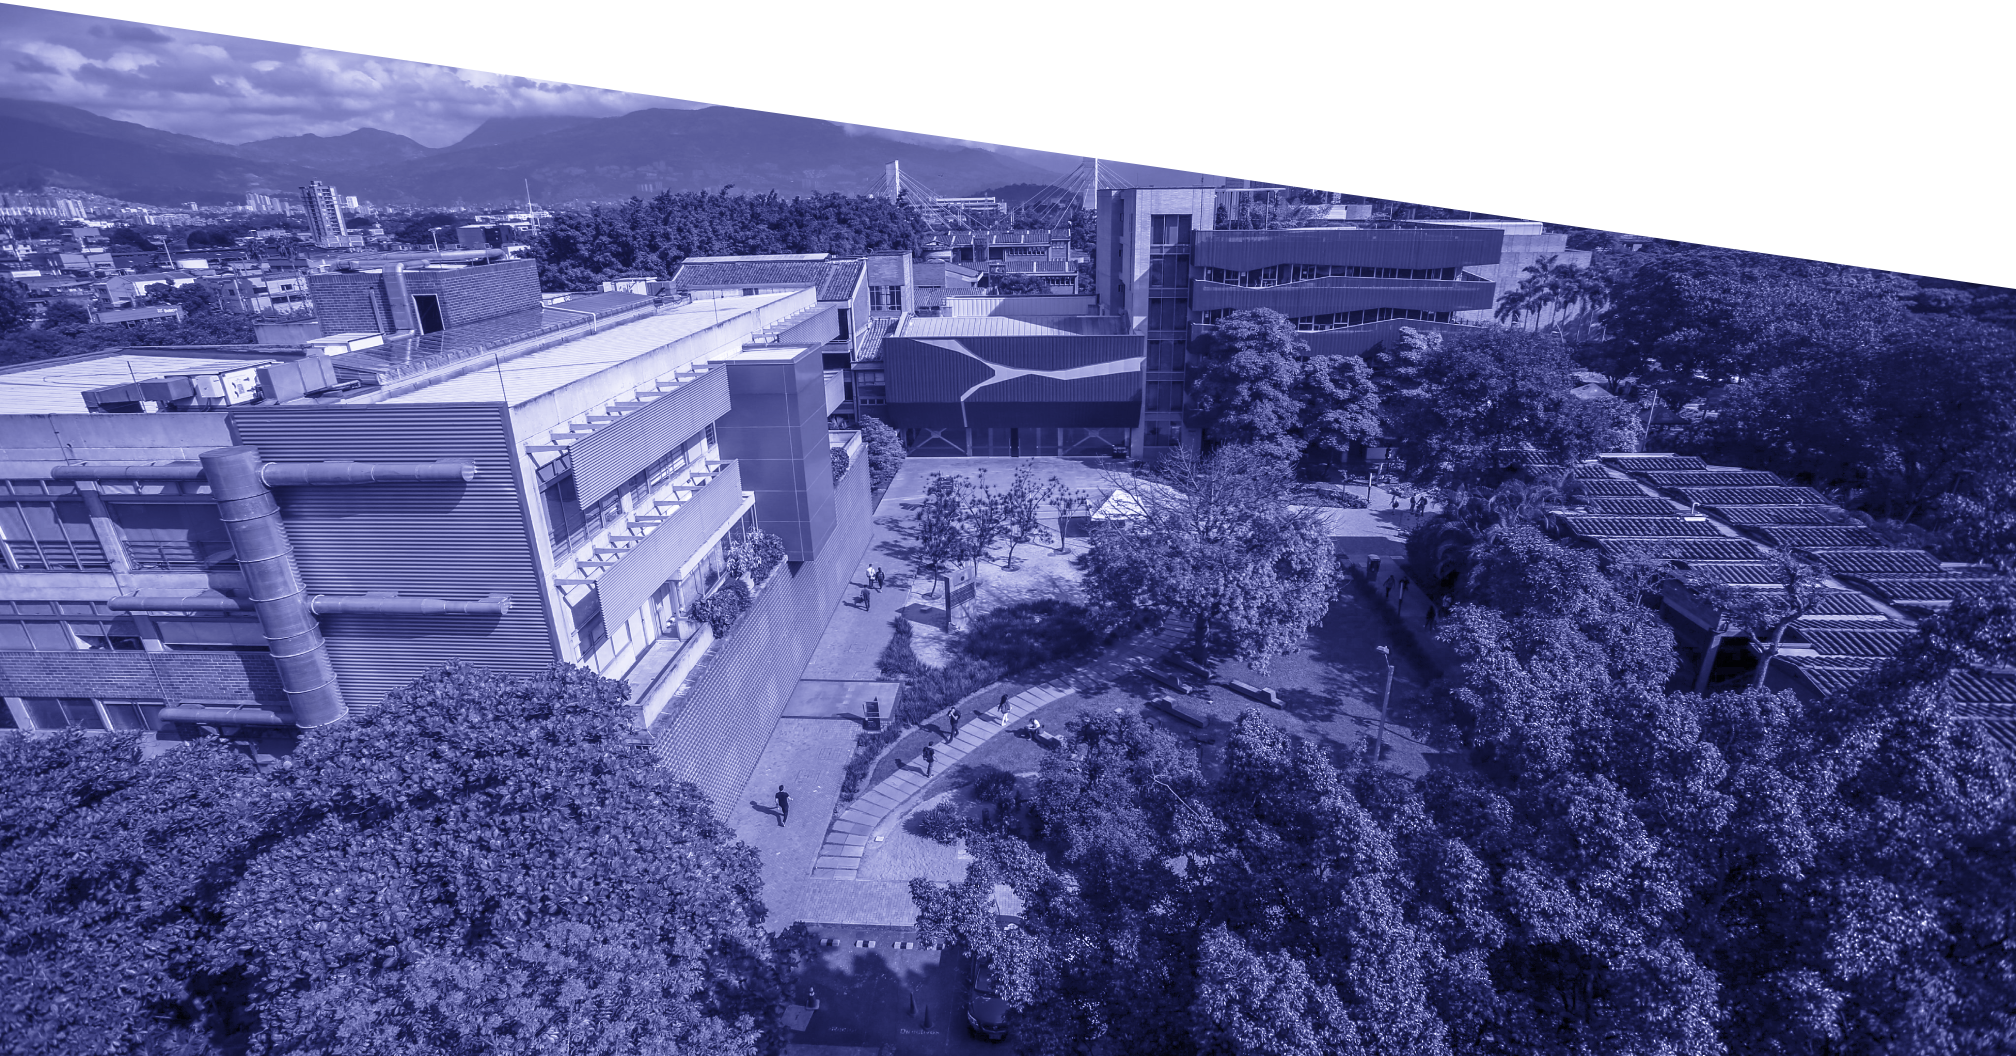
\includegraphics[width=\paperwidth]{Figures/0. General/eafit_banner.png}};

\mbox{}
\vfill
\sffamily \Large \textcolor{white}{\placeanddate} \\



\end{titlepage}









\newpage

% Generates a ToC without page number
{\hypersetup{linkcolor=black} % Keeps the ToC black even with non-black linkcolor
\tableofcontents\thispagestyle{empty}}
\newpage

% contains the introduction
\section{Introducción}

En el siguiente proyecto, nos embarcaremos en la tarea de diseñar e implementar
una infraestructura de red robusta y escalable para una empresa multinacional
que ha establecido su sede principal en la ciudad de Bogotá. Nuestro principal
objetivo será proporcionar una arquitectura de red que garantice un alto
rendimiento y una conectividad ininterrumpida, teniendo en cuenta la
expectativa de un alto volumen de tráfico para su página web.
\\

Procederemos a diseñar una topología de red en estrella, una estructura que se
destaca por su confiabilidad y capacidad para administrar eficientemente el
tráfico de red. Con este enfoque, cada sede de la empresa estará conectada a un
nodo central, en este caso, la sede principal en Bogotá, permitiendo una
comunicación fluida entre todas las localidades.
\\

La página web de la empresa será desplegada en un clúster de servidores web
para asegurar un rendimiento óptimo, incluso ante un alto tráfico. Esto no
solo mejorará la disponibilidad del sitio, sino que también ofrecerá una mayor
tolerancia a fallos y flexibilidad, ya que los recursos pueden ser ajustados de
acuerdo con la demanda.
\\

Además, como líder del equipo de infraestructura, estaré al frente de la
supervisión del despliegue, asegurándome de que todas las partes del sistema
funcionen en armonía y cumplan con las expectativas de la empresa.
\\

En el transcurso de este proyecto, describiré en detalle el proceso de diseño
de la topología de red, la implementación del clúster de servidores web, así
como las medidas que se tomarán para garantizar la seguridad, la escalabilidad
y la eficiencia de la infraestructura de red.
\\

Estoy convencido de que, al final de este trabajo, habremos creado una
infraestructura sólida y confiable que permitirá a la empresa operar su página
web de manera eficiente y sin interrupciones, sin importar la cantidad de
tráfico que reciba. \pagenumbering{arabic}
\newpage

% contains the project, but the static mode
\section{Proyecto Estático}

\subsection{VLSM}

Ahora bien, antes de comenzar a desarrollar e implementar nuestra solución,
lo mejor es definir completamente la infraestructura y primero usaremos
VLSM \textit{(Variable Length Subnet Mask)}. Entonces en la siguiente sección,
nos centraremos en un componente crítico de la gestión de redes: el Subneteo de
Longitud de Máscara Variable \textit{(Variable Length Subnet Masking, VLSM)}.
\\

VLSM es una técnica que permite dividir eficientemente el espacio de
direcciones IP en subredes de diferentes tamaños, según las necesidades
específicas de cada subred. Es una mejora significativa respecto al subneteo de
longitud de máscara fija, que obliga a todas las subredes a ser del mismo
tamaño, lo que puede resultar en una utilización ineficiente del espacio de
direcciones IP.
\\

En el contexto de nuestro proyecto, VLSM es esencial por varias razones.
Primero, nos permite maximizar el uso del espacio de direcciones IP asignado a
la empresa. Dado que las diferentes sedes y departamentos de la empresa pueden
tener diferentes necesidades en términos de cantidad de hosts requeridos, el uso
de VLSM nos permite asignar el espacio de direcciones de manera eficiente, 
minimizando el desperdicio.
\\

En segundo lugar, VLSM puede mejorar el rendimiento de la red al reducir la
cantidad de tráfico de enrutamiento innecesario. Al diseñar subredes que se
ajusten a las necesidades específicas de cada sede o departamento, podemos
minimizar la cantidad de tráfico de red que necesita ser enrutado a través de la
red principal, lo que a su vez puede mejorar el rendimiento general de la red.
\\

Finalmente, el uso de VLSM puede ayudar a mejorar la seguridad de la red. Al
segmentar la red en subredes de diferentes tamaños, podemos aplicar políticas
de seguridad más granulares, lo que nos permite tener un control más preciso
sobre quién puede acceder a qué partes de la red.
\\

En resumen, VLSM es una herramienta poderosa que nos permite diseñar e
implementar una red que es eficiente, segura y capaz de satisfacer las
necesidades específicas de la empresa (del ejercicio). En las siguientes
páginas, detallaremos cómo implementaremos VLSM en el diseño de nuestra red.
\\

Ahora bien, tenemos 7 redes de oficinas

\subsection{Implementación}

Ahora bien, para implementarlo realizamos lo siguiente:
\newpage

% contains the project, but the static mode
\section{Proyecto Dinámico}

\subsection{OSPF}

En este proyecto, uno de los aspectos fundamentales para garantizar la robustez
y la escalabilidad de nuestra infraestructura de red es la implementación de
una estrategia de enrutamiento eficiente. A lo largo de este trabajo, hemos
enfatizado la importancia del VLSM y el subnetting en el diseño de nuestra red.
Sin embargo, para añadir una capa adicional de eficiencia y flexibilidad, hemos
optado por implementar el Protocolo de Estado de Enlace Abierto
(Open Shortest Path First, OSPF).
\\

OSPF es un protocolo de enrutamiento de estado de enlace, que es especialmente
adecuado para redes de gran tamaño, como la que estamos diseñando para esta
empresa multinacional. Al combinarlo con nuestra estrategia de VLSM y
subnetting, y dada nuestra topología de red en estrella y el esperado alto
volumen de tráfico de la página web de la empresa, OSPF se presenta como una
solución ideal para gestionar eficazmente el tráfico de red y asegurar una
conectividad ininterrumpida.
\\

La importancia de OSPF en este proyecto radica en su capacidad para determinar
la ruta más corta y menos congestionada para el envío de paquetes de datos en
la red. Esto se logra mediante el algoritmo de Dijkstra, que OSPF utiliza para
calcular las rutas más eficientes. Esta capacidad es particularmente relevante
dada la estructura de nuestra red, que conecta todas las sedes de la empresa a
un nodo central, en este caso, la sede principal en Bogotá.
\\

Además, OSPF es un protocolo de enrutamiento dinámico, lo que significa que es
capaz de adaptarse rápidamente a los cambios en la red. En caso de un fallo de
red o un cambio en la topología de la red, OSPF puede ajustar rápidamente las
rutas de los paquetes de datos para evitar la interrupción de la conectividad.
Esta capacidad de recuperación y adaptabilidad, combinada con la flexibilidad
proporcionada por VLSM y subnetting, es esencial para mantener la disponibilidad
del sitio web de la empresa y garantizar un rendimiento óptimo,
independientemente del volumen de tráfico.
\\

En las siguientes secciones, detallaré cómo hemos implementado OSPF en nuestra
infraestructura de red, y cómo esta decisión, en combinación con el uso de VLSM
y subnetting, contribuye a los objetivos de robustez, escalabilidad y
eficiencia de nuestro diseño de red. Estamos convencidos de que, con la
implementación de OSPF, estaremos mejor equipados para enfrentar los desafíos
que presenta la gestión de una red de gran tamaño y alto tráfico.

\subsection{Implementación}

Como ya se sabe, nuestra infraestructura de red se basa en una topología de
estrella, donde la ciudad de Bogotá actúa como el nodo central o router
principal. Desde Bogotá, las conexiones se extienden a través de cables seriales
hacia las demás ciudades, que incluyen Medellín, Barranquilla, Rionegro, Cali,
Popayán, entre otras, mientras que las conexiones internas se gestionan mediante
cables ethernet.
\\

Es importante destacar que, a pesar de estar interconectados, cada uno de los
routers tiene un direccionamiento de red único. Este diseño incorpora un total
de 7 switches, cada uno de los cuales está conectado a 3 clientes, lo que suma
un total de 21 clientes en toda la red.
\\

Para cada router, asignamos una dirección IP y su correspondiente máscara de
subred. Con estas configuraciones, la puerta de enlace predeterminada
corresponde a la dirección IP configurada en los routers. Los switches, por otro
lado, actúan como puntos de conexión y, por lo tanto, no requieren configuraciones adicionales.
\\

Realizamos la configuración de los routers, específicamente el modelo 1841, a
través de la terminal. Asimismo, fue necesario añadir dos interfaces seriales a
la configuración de la interfaz web para garantizar una comunicación efectiva en
toda la red.

\newpage

% contains the conclusion of the project
\section{Conclusiones}

Para concluir, el diseño e implementación de la infraestructura de red para esta
empresa multinacional ha sido un proyecto desafiante pero sumamente
gratificante. Hemos logrado conceptualizar y poner en práctica una solución
robusta y escalable que no solo satisface las necesidades actuales de la
empresa, sino que también está preparada para adaptarse a su crecimiento futuro.
\\

La implementación de la topología de red en estrella ha proporcionado una
estructura confiable y eficiente para la gestión del tráfico de red. Al conectar
todas las sedes a un nodo central, hemos asegurado una comunicación fluida entre
todas las localidades, y la flexibilidad inherente a esta arquitectura nos
permitirá expandir y adaptar la red a medida que la empresa continúe creciendo.

\begin{figure}[H]
    \centering
    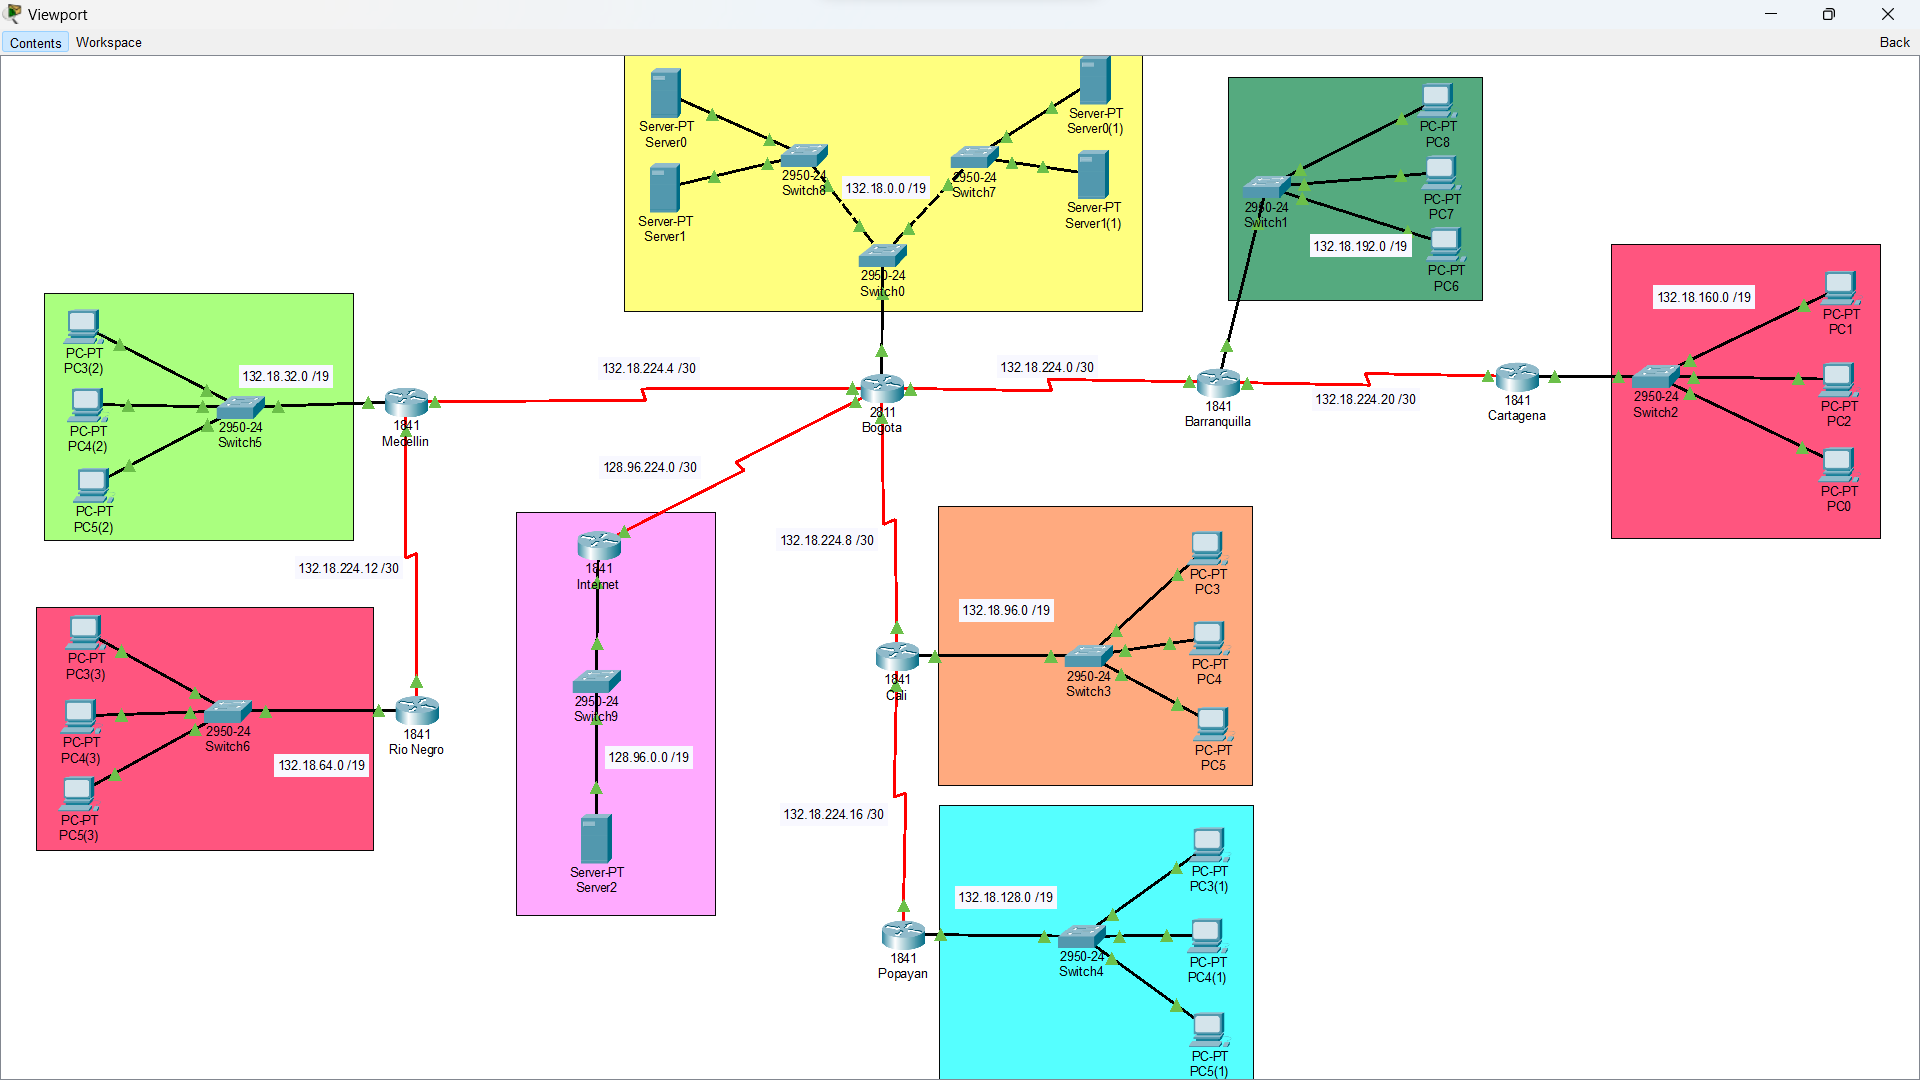
\includegraphics[width=0.7\textwidth]{Figures/4. Conclusions/final_result.png}
    \caption{Topología Completa de la red}
    \label{fig: Topologia Completa de la red}
\end{figure}

Además, el despliegue de la página web de la empresa en un clúster de servidores
web ha permitido manejar eficazmente un alto volumen de tráfico, garantizando un
rendimiento óptimo y una alta disponibilidad del sitio web. Esta solución ofrece
una gran tolerancia a fallos y permite ajustar los recursos de acuerdo con la
demanda, asegurando que la empresa pueda mantenerse al día con las necesidades
cambiantes de sus clientes.

\begin{figure}[H]
    \centering
    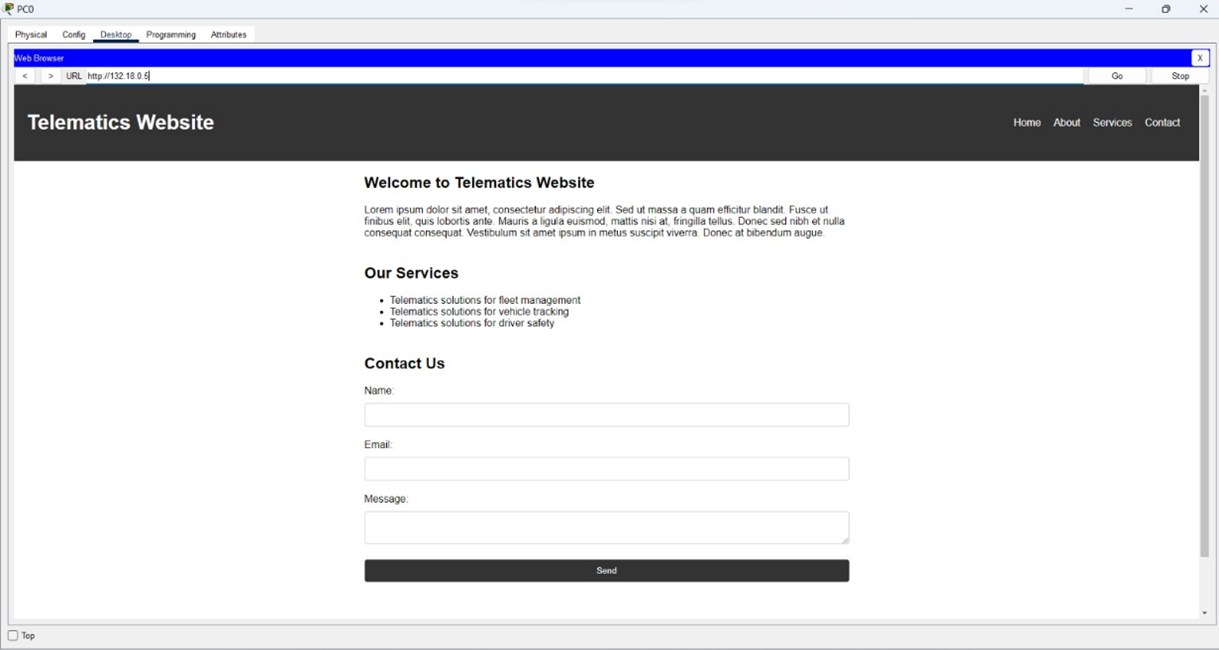
\includegraphics[width=0.7\textwidth]{Figures/4. Conclusions/web_page.png}
    \caption{Página web desplegada}
    \label{fig: deployed web page}
\end{figure}

\begin{figure}[H]
    \centering
    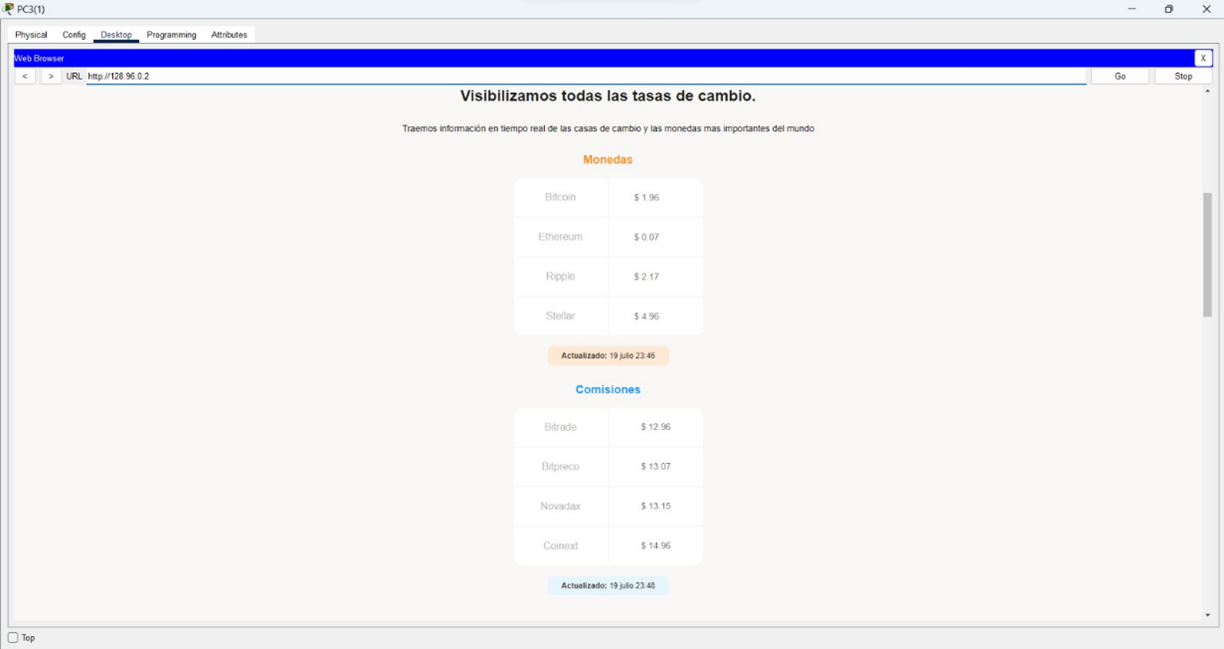
\includegraphics[width=0.7\textwidth]{Figures/4. Conclusions/internet_simulation.png}
    \caption{Simulación de acceso a internet}
    \label{fig: internet simulation}
\end{figure}

Además, la implementación de VLSM ha sido esencial para maximizar el uso del
espacio de direcciones IP y mejorar el rendimiento y la seguridad de la red. Al
permitir una asignación más eficiente del espacio de direcciones y políticas de
seguridad más granulares, VLSM ha demostrado ser una herramienta poderosa para
la gestión de redes.
\\

En una sección crucial de este proyecto, implementamos el Protocolo de Estado de
Enlace Abierto (Open Shortest Path First, OSPF) como nuestro protocolo de
enrutamiento dinámico. OSPF es un protocolo de enrutamiento de estado de enlace
que es ampliamente utilizado en redes de gran escala debido a su eficiencia,
escalabilidad y capacidad para recuperarse rápidamente ante fallos de red.
\\

La adopción de OSPF en nuestra infraestructura de red presenta varias ventajas
significativas. En primer lugar, OSPF es un protocolo de enrutamiento sin clase,
lo que significa que es compatible con VLSM y CIDR, permitiéndonos aprovechar
al máximo el espacio de direcciones IP disponible y mejorar la eficiencia de la
red.
\\

En segundo lugar, OSPF utiliza el algoritmo de Dijkstra para calcular la ruta
más corta a través de una red, lo que resulta en una gestión de tráfico
eficiente y efectiva. Este enfoque también garantiza una rápida convergencia de
la red en caso de fallos o cambios en la topología de la red, ya que cualquier
cambio en la topología se propaga rápidamente a través de la red.
\\

Además, OSPF admite el equilibrio de carga en múltiples rutas de igual costo, lo
que puede aumentar la disponibilidad y redundancia de la red. Esto es
especialmente útil en nuestra implementación, ya que nos permite manejar grandes
volúmenes de tráfico web de manera eficiente.
\\

Finalmente, OSPF es un protocolo de enrutamiento de código abierto, lo que
significa que no estamos atados a un proveedor específico de hardware de red y
tenemos una gran flexibilidad para adaptar y ajustar la configuración de la red
a nuestras necesidades específicas.
\\

Por lo tanto, la implementación de OSPF ha sido un componente clave para
asegurar una red robusta, resiliente y eficiente.
\\

En resumen, este proyecto ha sido un ejemplo de cómo un diseño de red cuidadoso
y una implementación eficaz pueden ayudar a una empresa a satisfacer sus
necesidades de conectividad, mejorar su rendimiento y asegurar su futuro
crecimiento. Estamos orgullosos de lo que hemos logrado y confiamos en que esta
infraestructura de red servirá bien a la empresa (del ejercicio) en los años 
venideros.
\newpage

% contains inspiration for formatting tables, images, text citations etc.
\section{This is a section}
\subsection{This is a subsection}

\subsubsection{This is a subsubsection}
This section contains some templates that can be used to create a uniform style within the document. It also shows of the overall formatting of the template, created using the predefined styles from the \texttt{settings.tex} file.

\subsection{General formatting}
Firstly, the document uses the font mlmodern, using no indent for new paragraphs and commonly uses the color \textcolor{EAFIT-blue}{EAFIT-blue} in its formatting. It uses the \texttt{fancyhdr} package for its headers and footers, using the EAFIT logo and report title as the header and the page number as the footer. The template uses custom section, subsection and subsubsection formatting making use of the \texttt{titlesec} package.\\
The \texttt{hyperref} package is responsible for highlighting and formatting references like figures and tables. For example \cref{table: style 1} or \cref{fig: three images}. It also works for citations \cite{texbook}. Note how figure numbers are numbered according to the format \texttt{<chapter number>.<figure number>}.\\

Bullet lists are also changed globally, for a maximum of 3 levels:

\begin{itemize}
    \item Item 1
    \item Item 2
    \begin{itemize}
        \item subitem 1
        \begin{itemize}
            \item subsubitem 1
            \item subsubitem 2
        \end{itemize}
    \end{itemize}
    \item Item 3
\end{itemize}

Similarly numbered lists are also changed document wide:

\begin{enumerate}
    \item Item 1
    \item Item 2
    \begin{enumerate}
        \item subitem 1
        \begin{enumerate}
            \item subsubitem 1
            \item subsubitem 2
        \end{enumerate}
    \end{enumerate}
    \item Item 3
\end{enumerate}

\newpage

\subsection{Tables and figures}
The following table, \cref{table: style 1}, shows a possible format for tables in this document. Alternatively, one can also use the black and white version of this, shown in \cref{table: style 2}. Note that caption labels are in the format \textbf{\textcolor{EAFIT-blue}{Table x.y:} }
\begin{table}[ht]
\rowcolors{2}{EAFIT-blue!10}{white}
\centering
\caption{A table without vertical lines.}
\begin{tabular}[t]{ccccc}
\toprule
\color{EAFIT-blue}\textbf{Column 1}&\color{EAFIT-blue}\textbf{Column 2}&\color{EAFIT-blue}\textbf{Column 3}&\color{EAFIT-blue}\textbf{Column 4}&\color{EAFIT-blue}\textbf{Column 5}\\
\midrule
Entry 1&1&2&3&4\\
Entry 2&1&2&3&4\\
Entry 3&1&2&3&4\\
Entry 4&1&2&3&4\\
\bottomrule
\end{tabular}
\label{table: style 1}
\end{table}

\begin{table}[ht]
\rowcolors{2}{gray!10}{white}
\centering
\caption{A table without vertical lines.}
\begin{tabular}[t]{ccccc}
\toprule
\textbf{Column 1}&\textbf{Column 2}&\textbf{Column 3}&\textbf{Column 4}&\textbf{Column 5}\\
\midrule
Entry 1&1&2&3&4\\
Entry 2&1&2&3&4\\
Entry 3&1&2&3&4\\
Entry 4&1&2&3&4\\
\bottomrule
\end{tabular}
\label{table: style 2}
\end{table}

For normal, single image figures, the standard \texttt{\textbackslash begin\{figure\}} environment can be used. For multi-image figures, one could use either the \texttt{\textbackslash begin\{subfigure\}} environment to get a main caption with 3 subcaptions like \cref{fig: three images} or the \texttt{\textbackslash begin\{minipage\}} environment to get 3 independent captions like \cref{fig: style 2 image a} - \ref{fig: style 2 image c}

\begin{figure}[H]
     \centering
     \begin{subfigure}[b]{0.3\textwidth}
         \centering
         \includegraphics[width=\textwidth]{example-image-a}
         \caption{image a}
         \label{fig: style 1 image a}
     \end{subfigure}
     \hfill
     \begin{subfigure}[b]{0.3\textwidth}
         \centering
         \includegraphics[width=\textwidth]{example-image-b}
         \caption{image b}
         \label{fig: style 1 image b}
     \end{subfigure}
     \hfill
     \begin{subfigure}[b]{0.3\textwidth}
         \centering
         \includegraphics[width=\textwidth]{example-image-c}
         \caption{image c}
         \label{fig: style 1 image c}
     \end{subfigure}
        \caption{Three images}
        \label{fig: three images}
\end{figure}

\begin{figure}[H]
\centering
\begin{minipage}{0.3\textwidth}
  \centering
  \includegraphics[width=\textwidth]{example-image-a}
  \captionof{figure}{image a}
  \label{fig: style 2 image a}
\end{minipage}
\hfill
\begin{minipage}{0.3\textwidth}
  \centering
  \includegraphics[width=\textwidth]{example-image-b}
  \captionof{figure}{image b}
  \label{fig: style 2 image b}
\end{minipage}
\hfill
\begin{minipage}{0.3\textwidth}
  \centering
  \includegraphics[width=\textwidth]{example-image-c}
  \captionof{figure}{image c}
  \label{fig: style 2 image c}
\end{minipage}
\end{figure}
\newpage

% Creates references using the Biblatex 
\bibliographystyle{plain}
\bibliography{General/References.bib}
\newpage

\end{document}
